\documentclass[runningheads]{llncs}
\usepackage[T1]{fontenc}
\usepackage{graphicx}
% Used for displaying a sample figure. If possible, figure files should
% be included in EPS format.
%
% If you use the hyperref package, please uncomment the following two lines
% to display URLs in blue roman font according to Springer's eBook style:
% \usepackage{hyperref}
% \usepackage{color}
% \renewcommand\UrlFont{\color{blue}\rmfamily}

\begin{document}

\title{Fairness analysis and machine learning model implementation
    using New Zealand prosecution and conviction data}

\titlerunning{Exploring fair classifiers on New Zealand criminal data}

\author{Fabio Garcia \and Pierre Omidyar \and Luis Rodrigues \and
    Junjie Xie}

\authorrunning{F. Garcia et al.}

\institute{University of Auckland, Auckland, New Zealand \\
    \email{\{fgar174, pomi601, lrdo555, jxie936\}@aucklanduni.ac.nz}}

\maketitle

\begin{abstract}
    In the era of data-driven decision-making, ensuring fairness in
    machine learning models is crucial, especially when the
    implications directly affect human lives. This research delves
    into the realm of fairness in machine learning, focusing on the
    potential biases that may arise when models are trained on
    sensitive attributes, particularly ethnicity. Utilizing a
    comprehensive dataset on conviction and prosecution from New
    Zealand, we aim to understand any bias in the data and evaluate
    the performance of models when sensitive attributes are
    considered. Preliminary findings indicate that models trained
    without proper fairness interventions exhibit significant
    disparities in predictions across different ethnic groups. This
    paper presents methodologies to mitigate such biases with the use
    of the toolkit AI Fairness 360~\cite{bellamy2018ai}, focusing on
    building and analysing machine learning models that can be
    considered fair according to the corresponding metrics. The
    results underscore the importance of incorporating fairness
    techniques in the machine learning pipeline, especially when
    dealing with critical domains like the justice system.
\end{abstract}

%%%%%%%%%%%%%%%%%%%%%%%%%%%%%%%%%%%%%%%%%%%%%%%%%%%%%%%%%%%%%%%%%%%%%%
\section{Introduction}
\label{sec:introduction}

Promoting fairness in machine learning, especially in crucial areas
such as the legal system, is vital. As decisions increasingly rely on
data, there's a growing concern about potential biases, especially
when models use sensitive factors like ethnicity for training. Given
New Zealand's varied ethnic makeup, it presents a distinctive
opportunity to study these biases, notably the differences between the
European and Ma\=ori communities, among others.

In our study, we explore fairness in machine learning by analysing two
extensive datasets from New Zealand: one on prosecution and the other
on conviction records. These datasets offer valuable insights into the
outcomes of model predictions when considering sensitive factors,
particularly ethnicity.

To provide a comprehensive analysis, we employed a variety of machine
learning models, including logistic regression, decision tree, random
forest, and k-nearest neighbour. Our evaluation metrics encompassed
disparate impact \cite{feldman2015certifying}, equalised odds
\cite{hardt2016equality}, precision, and accuracy. These metrics were
chosen due to their relevance in assessing fairness and performance in
predictive models, especially in the context of the criminal justice
system \cite{caton2020fairness,%
    chouldechova2017fair,corbett2017algorithmic}. The base group for
our analysis was the European ethnicity, with every other ethnicity
serving as the comparison group. This choice reflects the demographic
realities of New Zealand and allows for a nuanced exploration of
differences in outcomes experienced by certain ethnicities,
highlighting potential biases against minority groups.

The overarching goal of this research is not only to identify biases
but also to suggest methodologies to mitigate them, ensuring that
machine learning models are both accurate and fair. The integration of
fairness mitigations in the machine learning pipeline is crucial,
especially when dealing with critical domains like the justice system.
By focusing on New Zealand's prosecution and conviction data, this
study contributes to the growing body of literature on fairness in
machine learning, offering insights that could be instrumental in
shaping future policies and practices.

%%%%%%%%%%%%%%%%%%%%%%%%%%%%%%%%%%%%%%%%%%%%%%%%%%%%%%%%%%%%%%%%%%%%%%
\section{Related work}
\label{sec:related-work}

Critical reviews of fairness in machine learning, including trade-offs
between fairness and accuracy of classification models, can be found
in \cite{corbett2018measure} and \cite{romei2014multidisciplinary}.

Much of the recent scholarship on fairness in machine learning when
applied to criminal data followed the publication of an article by
U.S. journalists Julia Angwin et al.\ in \cite{angwin2016machine}.
They studied a risk prevention instrument by the company Northpointe
Inc. called COMPAS~\cite{compascore} and concluded it was biased
against black defendants. This finding was challenged by the company
in \cite{dieterich2016compas}. The publication raised a number of
issues and criticisms, and these are explored formally in
\cite{chouldechova2017fair}.

Many different methods have been proposed to quantify the level of
unfairness that exists in a dataset or a machine learning classifier.
Individual fairness and statistical parity are explored in
\cite{dwork2012fairness}. Equalised odds, equal opportunity and
demographic parity are further defined in \cite{hardt2016equality}.
The concept of disparate impact comes from U.S. law but is formalised
for use in machine learning in \cite{feldman2015certifying}.

When working with real world datasets related to criminal justice,
sources of bias in the raw data are a real concern.
\cite{suresh2019framework} explores the issues of historical bias,
representation bias and measurement bias. Data bias and algorithmic
bias are surveyed extensively in \cite{mehrabi2021survey}.

Several authors have applied fairness mitigations to criminal data.
\cite{corbett2017algorithmic,zafar2017fairness} explore the training
of fair classifiers on U.S. criminal data.

In the New Zealand context, \cite{rodger2023explainable} explores
sentencing prediction on New Zealand assault convictions using natural
language processing techniques, but does not explore fairness
mitigations.

Fair classifiers may suffer from reduced accuracy if measured against
test data where sensitive attributes are an important part of the
model. \cite{dressel2018accuracy} finds that a simple linear
classifier with only two features can match predictions made by the
COMPAS software.

In this work we explore several methods from the literature to remove
or mitigate bias present in our datasets. Disparate impact remover is
due to \cite{feldman2015certifying}. Reweighing is due to
\cite{kamiran2012data}. Grid search reduction is due to
\cite{agarwal2018reductions}. Calibrated equalised odds
post-processing is due to \cite{chouldechova2017fair}.

The toolkit AI Fairness 360~\cite{bellamy2018ai} provides a large
suite of tools to experiment with many of the fairness algorithms
developed by researchers and was central to the work we present here.
Others have built toolkits on top of AIF360, including
\cite{johnson2022fairkit}.

Finally, evaluation of machine learning models involves the extensive
use of performance metrics. The toolkit scikit-learn
\cite{scikit-learn} provides a large variety of performance metrics.


%%%%%%%%%%%%%%%%%%%%%%%%%%%%%%%%%%%%%%%%%%%%%%%%%%%%%%%%%%%%%%%%%%%%%%
\section{Methodology}
\label{sec:methodology}
In this section, we first introduce formal definitions of the metrics
we used, then describe our datasets and finally introduce formal
definitions of the fairness mitigations we applied. We then introduce
the AI Fairness 360 \cite{bellamy2018ai} library and the toolkit we
built on top of it, which is available on GitHub.%
\footnote{\url{https://github.com/Luchiwards/P2.FairnessResearchNZ}}


%%%%%%%%%%%%%%%%%%%%%%%%%%%%%%%%%%%%%%%%
\subsection{Disparate impact}
\label{sec:disparate-impact}

Disparate impact in machine learning refers to unintentional
discrimination in algorithmic outcomes.

Below is a formal description of disparate impact following the
definitions in \cite{feldman2015certifying,zafar2017fairness}:

\begin{enumerate}
\item \textbf{Protected Group}: A protected group is a set of
    individuals who share a specific protected characteristic, such as
    race, gender, religion, or age.

\item \textbf{Decision or Prediction}: Refers to the outcome or
    classification assigned by a model to a particular individual,
    such as approving or denying a loan application, hiring or not
    hiring a job applicant, or predicting the likelihood of recidivism
    for a criminal defendant.

\item Let $D = (X, Y, C)$ be a dataset, where $X$ is the protected
    attribute (e.g., race, sex, religion, etc.). $Y$ represents the
    remaining attributes. $C$ is the binary class to be predicted
    (e.g., ``will hire'').


    We say that $D$ has disparate impact if the following condition
    holds:
    \begin{equation}
        \frac{P(C = \mbox{YES} | X = 0)}{P(C = \mbox{YES} | X = 1)} \leq \tau = 0.8
    \end{equation}

    Here, $P(C = c | X = x)$ denotes the conditional probability,
    evaluated over $D$, that the class outcome is $c \in C$ given the
    protected attribute $x \in X$.
    % This condition compares the probability of a positive outcome
    % ($C = \mbox{YES}$) for the group with the protected attribute
    % value of 0 to the group with the protected attribute value of 1
    % and checks if the ratio is less than or equal to a threshold
    % value ($\tau$), which is set to 0.8 in this context. If the
    % ratio is less than or equal to 0.8, it indicates the presence of
    % disparate impact.

\end{enumerate}

%%%%%%%%%%%%%%%%%%%%%%%%%%%%%%%%%%%%%%%%
\subsection{Equalised odds}
\label{sec:equalised-odds}

A predictor $Y_b$ satisfies equalised odds \cite{hardt2016equality}
with respect to a protected attribute $A$ and outcome $Y$ if $Y_b$ and
$A$ are independent conditional on $Y$.

Equalised odds permits the use of features that directly predict $Y$
but prohibits the abuse of $A$ as a proxy for $Y$.

Equalised odds applies to a wide range of settings, including binary,
multi-class, continuous, or structured outcomes. However, in this
study we focus on the case of binary random variables $Y$, $Y_b$, and
$A$. In this case, equalised odds can be expressed as follows:

For $Y = 1$, the constraint requires that $Y_b$ has equal true
positive rates across the two demographics $A = 0$ and $A = 1$:
\[
    P(Y_b = 1 | A = 0, Y = 1) = P(Y_b = 1 | A = 1, Y = 1)
\]

For $Y = 0$, the constraint equalizes false positive rates:
\[
    P(Y_b = 1 | A = 0, Y = 0) = P(Y_b = 1 | A = 1, Y = 0)
\]


The definition aligns well with the goal of building highly accurate
classifiers. $Y_b = Y$ is always an acceptable solution, but
equalised odds enforces that the accuracy is equally high in all
demographics. Models that perform well only on the majority group are
penalized.

%%%%%%%%%%%%%%%%%%%%%%%%%%%%%%%%%%%%%%%%
\subsection{Datasets}
\label{sec:datasets}

We used two datasets for our analysis: New Zealand Police data on
proceedings against offenders%
\footnote{\url{https://www.police.govt.nz/about-us/publications-statistics/data-and-statistics/policedatanz/proceedings-offender-demographics}
    Retrieved 20 October 2023.}, and New Zealand Ministry of Justice
conviction and sentencing data.%
\footnote{\url{https://nzdotstat.stats.govt.nz/wbos/Index.aspx?DataSetCode=TABLECODE7373}
    Retrieved 20 October 2023.}

The Police data contains proceeding information against unique
offenders in the given period and covers the period from July, 2014
through July, 2023. The ``Method of Proceeding'' records Police
decision relating to a particular offender for the given offence.
Examples of values in this column are ``Court Action'', ``Formal
Warning'', and ``Informal Warning''.

The Justice data contains sentencing information for adults convicted
across New Zealand for the years 2001--2022. Examples of values in
this column are ``Community Detention'', ``Imprisonment'', and
``Intensive Supervision''.

Each dataset contained the following sensitive attributes: Age range
(in 5 year bands), Sex, and Ethnicity.

Offences are categorised using the Australian and New Zealand Standard
Offence Classification (ANZSOC)%
\footnote{\url{https://www.abs.gov.au/statistics/classifications/australian-and-new-zealand-standard-offence-classification-anzsoc/latest-release}
    Retrieved 20 October 2023.} There are sixteen top level
``divisions'' which are further subdivided into ``subdivisions'' and
``groups''. Figures~\ref{fig:justice-di} and \ref{fig:police-di} in
Section~\ref{sec:data-analysis} display fifteen of the sixteen main
divisions (excluding Traffic Offences).

Only the most serious offence by the offender is recorded in these
datasets.

\subsubsection{Data preparation}
The datasets present an aggregated view of the underlying operational
records. Each row contains an offence, a resolution (e.g.\ the type of
sentence received for the Justice data, or the referral to prosecution
or informal warning for Police), date, demographic attributes and a
count. In order to put the data in a standard format, we duplicated
each row according to its count, so that the total number of rows
matched the sum of the counts.

The datasets contain overlapping aggregated information, so special
care was required to avoid duplicating records. Each row contains the
count of sentences received by offenders with particular demographic
information in the given period, along with the ANZSOC offence code.
However, since ANZSOC is a hierarchical classification, a unique
offender is represented in three separate rows: one for the ANZSOC
Group of the offence, one for the Subdivision of the offence, and one
for the Division of the offence.

Accordingly, we subset the data appropriately given the task at hand.
For a high level analysis of the probability distributions of
sentences by ethnicity, we subset the data to select the sixteen top
level ANZSOC Divisions. For training machine learning models, we
subset the data to use the most specific level (Group or Subdivision)
available for each Division.

For both datasets, we eliminated the following rows:
\begin{itemize}
\item All offences in the Traffic and Vehicle Regulatory Offences
    division
\item All rows where ethnicity was Other, Not Stated, Not Elsewhere
    Classified, or Unknown
\item All rows where the sentence was No Sentence Recorded
\end{itemize}

These datasets are feature-poor. In addition to the ANZSOC
classification of the offence, they provide only three attributes, all
of which are sensitive: age, gender, and ethnicity. Despite this, as
we will see in Section~\ref{sec:model-implementation} Model
implementation, several classifiers achieve high accuracy.

After these preparations, the Justice dataset had 1,497,315 records,
and the Police dataset had 1,024,104.

Prior to their use as training data, one additional step was performed
on the Justice data: the removal of highly unbalanced offences. For
each offence category, for number of instances less than 100 rows or
if the ratio of imprisonment to non-imprisonment offences was
$< 0.25$, the data was removed. This approach followed
\cite{ali2019imbalance}. The remaining number of rows in that dataset
was 314,230.


%%%%%%%%%%%%%%%%%%%%%%%%%%%%%%%%%%%%%%%%
\subsection{Mitigations}
\label{sec:mitigations}

We explored several mitigation algorithms. They are described in this
section.

\subsubsection{Disparate impact remover}
This mitigation proposed by \cite{feldman2015certifying} aims to
reduce disparate impact (Section~\ref{sec:disparate-impact}) present
in a model.

\paragraph{Input} The Disparate Impact Remover takes the following
inputs:
\begin{itemize}
\item A dataset $D = (X, Y, C)$ consisting of features ($X$), target
    labels ($Y$), and a sensitive attribute ($C$).
\item A binary classification model $M$ trained to predict the target
    labels ($Y$).
\end{itemize}

\paragraph{Principles of operation} For each \(Y\) value in the
dataset (\(y \in Y_x\)), all of them generate the corresponding
repaired \(\bar{Y}\) value (\(\bar{y} = F^{-1}_A(F_x(y))\)) to ensure
more equal performance among different groups. This transformation
exclusively modifies the \(Y\) attribute, leaving the protected
attribute \(X\) and the class \(C\) unaffected, ensuring that the
model can still accurately predict class labels.

\subsubsection{Reweighing}
This mitigation is proposed by \cite{kamiran2012data}. It involves
adjusting the weights assigned to different instances in a dataset to
balance the impact of sensitive attributes on model predictions.

\paragraph{Input} The Reweighing technique takes the following inputs:
\begin{itemize}
\item A dataset $D = (X, Y, C)$ consisting of features ($X$), target
    labels ($Y$), and a sensitive attribute ($C$).
\item A binary classification model $M$ trained to predict the target
    labels ($Y$).
\end{itemize}

\paragraph{Principles of operation} Reweighing reallocates sample
weights for different classes to balance their importance. Classes
with fewer samples are assigned higher weights, while those with more
samples are assigned lower weights. This helps ensure that during
model training, minority classes are not overlooked.

\subsubsection{Calibrated equalised odds}
Calibrated Equalised Odds Post-processing (CEOP) is proposed by
\cite{pleiss2017fairness}. It adjusts the predicted probabilities of a
model to satisfy the Equalised Odds fairness criterion while
maintaining overall model performance.

\paragraph{Input} CEOP takes the following inputs:
\begin{itemize}
\item A binary classification model $M$ trained to predict target
    labels.
\item A validation dataset $V = (X, Y, C)$ consisting of features
    ($X$), true labels ($Y$), and sensitive attributes ($C$).
\item A test dataset $T = (X', Y', C')$ with similar characteristics
    as the validation dataset.
\end{itemize}

\paragraph{Principles of operation}
CEOP uses equalised odds (Section~\ref{sec:equalised-odds}) to
calculate the difference in $TPR$ and $FPR$ between groups.

The model's prediction thresholds are then calibrated to ensure that
each group performs similarly.

%%%%%%%%%%%%%%%%%%%%%%%%%%%%%%%%%%%%%%%%
\subsection{AI Fairness 360}
\label{sec:ai-fairness-360}

AI Fairness 360 \cite{bellamy2018ai}, is an open-source toolkit
developed by IBM that provides a comprehensive set of algorithms and
tools to help researchers address and mitigate bias and fairness
issues in machine learning models. It offers many pre-processing and
post-processing techniques to detect and reduce bias in data and model
predictions.

\subsection{Our toolkit}
\label{sec:our-toolkit}

This research adopts an experimental methodology shown in
Figure~\ref{fig:methodology-workflow}, aiming to assess the impact of
fairness mitigations on models including an analysis of the trade-off
between accuracy and fairness. Using the AIF360 toolkit, our study
evaluates preprocessing and post-processing interventions on our
datasets. See footnote in Section~\ref{sec:methodology} for GitHub
link.

\begin{figure}
    \centering 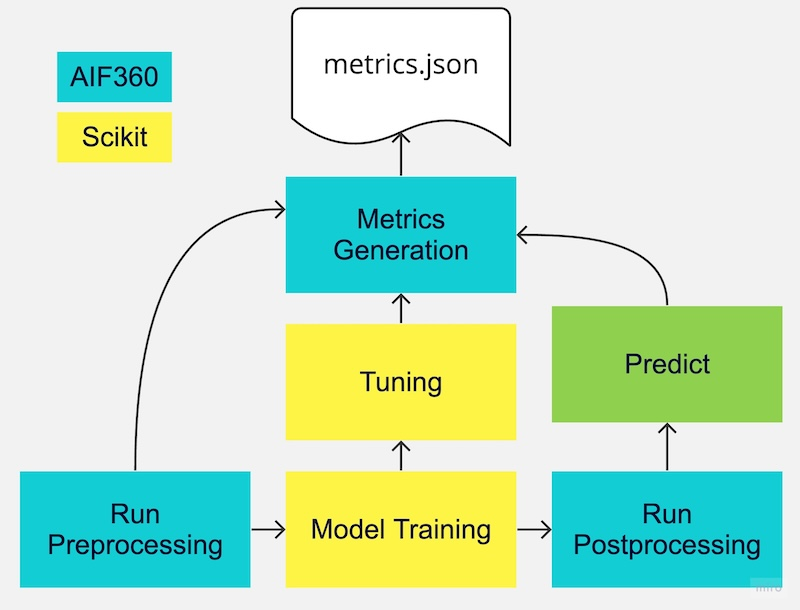
\includegraphics[width=0.5\textwidth]{../tex/Flowchart}
    \caption{Process Workflow}
    \label{fig:methodology-workflow}
\end{figure}

% \subsubsection{Dataset and Preprocessing}

% The datasets used in our study are described in
% Section~\ref{sec:datasets}.

% To initiate the process for both datasets, custom dataset classes
% were created in line with the structure provided by the AIF360
% library.

\subsubsection{Workflow and Configuration}

The main workflow for our fairness intervention is encapsulated within
a \texttt{FairnessProcessMitigation} object, which is called from
either the \texttt{run\_police} or \texttt{run\_justice} files,
specific to each dataset.

The process is executed as follows:
\begin{description}
\item[Dataset Splitting] The dataset (either police or justice) is
    split into a training set and a test set, with a 70\%-30\% ratio,
    using a consistent random seed for reproducibility.

\item[Preprocessing] Before training the models, any specified
    preprocessing strategies are executed. These could be a
    combination of strategies, such as Reweighing (PRW) and Disparate
    Impact Remover (PDIR).

\item[Model Training and Evaluation] The specified models are trained
    on the preprocessed training data. During training, a grid search
    is conducted to determine the best hyper-parameters for each
    model. The performance and training details (e.g., best
    parameters, feature importance) of each model are stored in the
    \texttt{metrics.json} file.

\item[Post-Processing] Once models are trained and have made
    predictions, a post-processing phase is initiated, if specified.
    The available post-processing option is the Calibrated Equalised
    Odds (PTCO). Model predictions are adjusted in this phase to
    further enhance fairness.

\item[Metrics Storage] All relevant metrics, including disparate
    impact and statistical parity differences for both the overall
    dataset and individual ethnicities, are stored in the
    \texttt{metrics.json} file. This allows for comprehensive post-hoc
    analysis and comparisons between models and mitigation strategies.
\end{description}

\subsubsection{Metrics and Results Storage}

The \texttt{metrics.json} file provides a structured storage mechanism
for the outcomes of the process. The primary structure of this file is
based on a combination of the database's name and the mitigation
nomenclature. Under this primary key, metrics related to dataset
fairness (e.g., disparate impact) and individual model performance
(e.g., accuracy, precision) are stored. This structure allows for
efficient retrieval and analysis of results.

\subsubsection{Considerations}

The entire process adopts specific nomenclatures to denote the
mitigation techniques employed:
\begin{description}
\item[NM:] for No Mitigation
\item[PRW:] for Reweighing
\item[PDIR:] for Disparate Impact Remover
\item[PTCO:] for Calibrated Equalised Odds in post-processing
\end{description}

By using these nomenclatures, we ensure a consistent and easily
understandable representation of the mitigation strategies across all
phases of our study.



%%%%%%%%%%%%%%%%%%%%%%%%%%%%%%%%%%%%%%%%%%%%%%%%%%%%%%%%%%%%%%%%%%%%%%
\section{Results}
\label{sec:results}

\subsection{Data analysis}
\label{sec:data-analysis}
In order to quantify the level of data bias \cite{mehrabi2021survey}
present in our datasets, we compared the base rates of severe outcomes
for similar crime categories when partitioned by ethnicity, which
corresponds to the notion of \emph{statistical parity} as in
\cite{corbett2017algorithmic}. This is sometimes also called
\emph{demographic parity} in the literature.

We defined severe outcomes in the following way: for police data on
prosecution decisions, a severe outcome was an offender being referred
to prosecution. For court data on convictions, a severe outcome was an
imprisonment sentence.

For statistical parity, the expected rate of severe outcome
conditioned on each subgroup ought to equal to the overall expected
rate of severe outcome, i.e.
\begin{equation}
    \label{eq:parity}
    P(Y = 1 | X = 0) = P(Y = 1 | X = 1)
\end{equation}
where $Y = 1$ indicates the less severe outcome, $X = 1$ indicates the
base subgroup (e.g.\ European in our analysis), and $X = 0$ indicates
the comparison subgroup (non-European in our analysis).

\emph{Disparate impact} is simply this equality (\ref{eq:parity})
expressed as a ratio \cite{feldman2015certifying}:
\begin{equation}
    \label{eq:disparate-impact}
    \frac{P(Y = 1 | X = 0)}{P(Y = 1 | X = 1)}
\end{equation}

Figure~\ref{fig:justice-di} shows the disparate impact measured in the
conviction dataset for the years 2001-2022. As discussed in
\cite{chouldechova2017fair,mehrabi2021survey}, bias evident in a
dataset like this cannot necessarily be attributed to human bias. We
made no attempt to investigate possible explanations for the
difference in probability distributions among these ethnicities.

No matter the cause, this type of uneven distribution poses challenges
to machine learning models trained on this data
\cite{feldman2015certifying}. Note that the symbol size in the figures
are proportional to the population size, so the uneven distribution
represents a challenge to balancing the dataset.

Figure~\ref{fig:police-di} shows a similar analysis of the dataset
containing police referrals to prosecution. Here we see a wider range
of disparate impact scores, including many receiving more favourable
outcomes than the base group.

\begin{figure}
    \centering
    \includegraphics[width=0.8\textwidth]{../justice-disparate-base-2001-2022}
    \caption{Disparate impact of imprisonment sentences, 2001-2022}
    \label{fig:justice-di}
\end{figure}
\begin{figure}
    \centering
    \includegraphics[width=0.8\textwidth]{../police2-disparate-base}
    \caption{Disparate impact of prosecution referrals, 2014-2023}
    \label{fig:police-di}
\end{figure}


%%%%%%%%%%%%%%%%%%%%%%%%%%%%%%%%%%%%%%%%
\subsection{Model implementation}
\label{sec:model-implementation}
Using the toolkit we developed and described in
Section~\ref{sec:our-toolkit}, we trained several models and evaluated
them using several fairness metrics, then applied several mitigations
and compared the effectiveness of those mitigations.

\subsubsection{Police dataset}
Figure~\ref{fig:police-di-mitigation} shows disparate impact scores
before mitigations (left panel) and after (right panel).
Figure~\ref{fig:police-acc-mitigation} shows accuracy scores before
mitigations and after.

Before mitigation, all models displayed accuracy scores over 70\% for
each ethnicity.
After mitigation, disparate impact significantly improved, especially
in gradient boosting and logistic regression models.
However, the accuracy suffered, with rates dropping below 30\% in the
best scenarios and plummeting to around 17\% in the worst.

Figure~\ref{fig:police-eqq-mitigations} shows equalised odds for
logistic regression, before mitigations and after.
The equalized odds changed significantly, increasing the recall while
dropping the precision.

\begin{figure}
    \begin{minipage}{0.52\textwidth}
        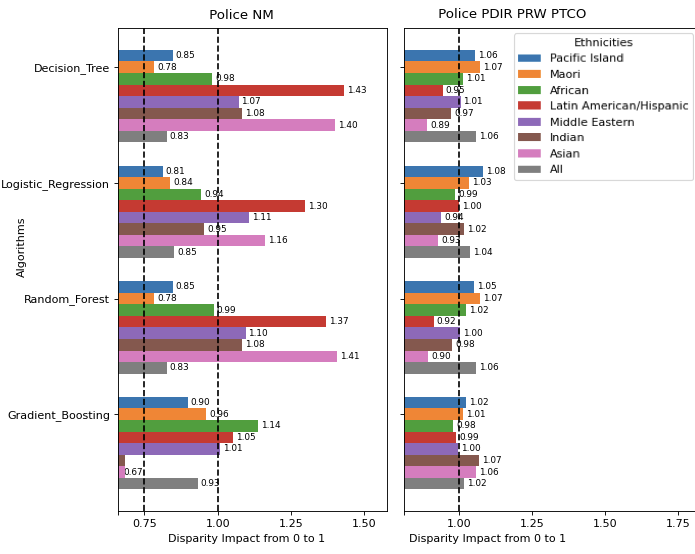
\includegraphics[width=\textwidth]{../tex/police_di_1_2}
        \caption{Police: disparate impact, before/after}
        \label{fig:police-di-mitigation}
    \end{minipage}
    \begin{minipage}{0.47\textwidth}
        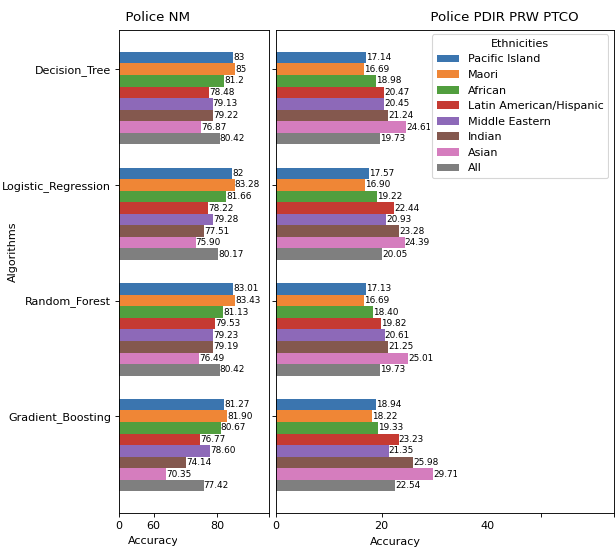
\includegraphics[width=\textwidth]{../tex/police_acc_1_2}
        \caption{Police: accuracy, before/after}
        \label{fig:police-acc-mitigation}
    \end{minipage}
\end{figure}

\begin{figure}
    \centering
    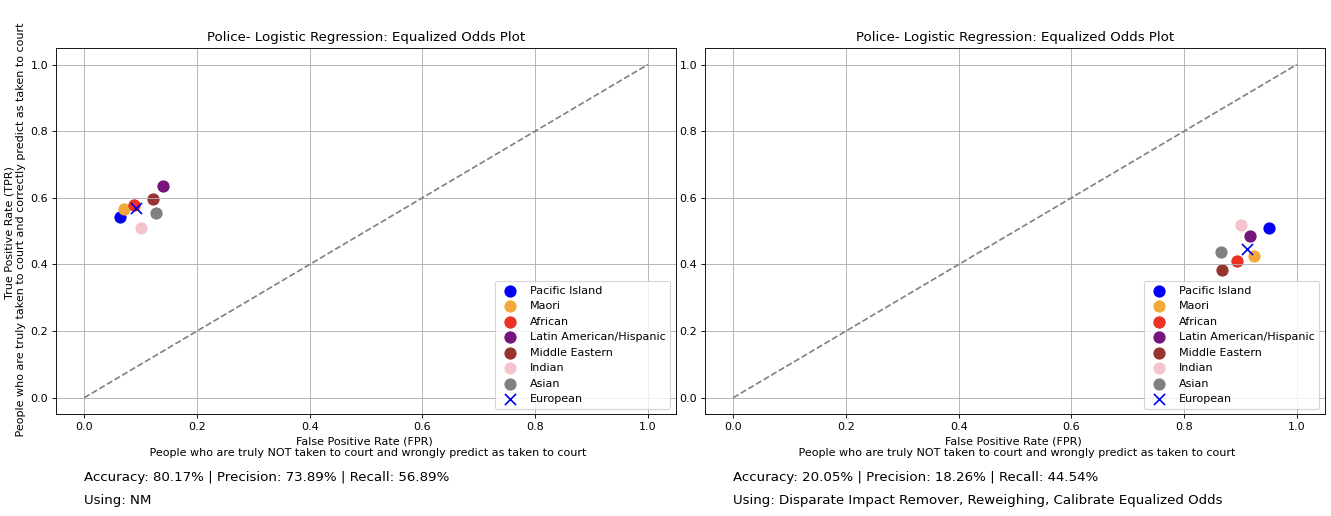
\includegraphics[width=\textwidth]{../tex/police_eqq}
    \caption{Police: equalised odds, before/after}
    \label{fig:police-eqq-mitigations}
\end{figure}

\subsubsection{Justice dataset}
Figure~\ref{fig:justice-di-mitigations} shows disparate impact scores
before mitigations and after.
Figure~\ref{fig:justice-acc-mitigations} shows accuracy scores before
mitigations and after.

Before mitigation, model accuracy ranged between 58\% and 69\%.
After mitigation, accuracy declined to around 30\% for some
ethnicities, with a peak at about 55\%.
After mitigation, disparate impact improved in the logistic regression
and K nearest neighbours models. However, the K nearest neighbours model
exhibited a concerning trend: predicting incarceration for all
ethnicities indiscriminately.

Figure~\ref{fig:justice-eqq-mitigations} shows equalised odds before
mitigation and after. Equalised odds changed significantly, increasing
the recall while dropping the precision.

\begin{figure}
    \begin{minipage}{0.55\textwidth}
        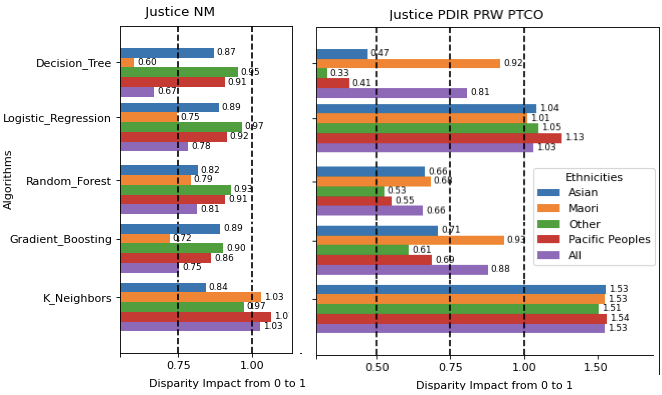
\includegraphics[width=\textwidth]{../tex/justice_di_1_2}
        \caption{Justice: disparate impact, before/after}
        \label{fig:justice-di-mitigations}
    \end{minipage}
    \begin{minipage}{0.44\textwidth}
        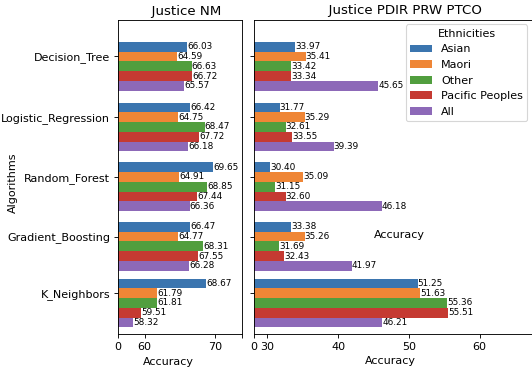
\includegraphics[width=\textwidth]{../tex/justice_acc_1_2}
        \caption{Justice: accuracy, before/after}
        \label{fig:justice-acc-mitigations}
    \end{minipage}
\end{figure}

\begin{figure}
    \centering
    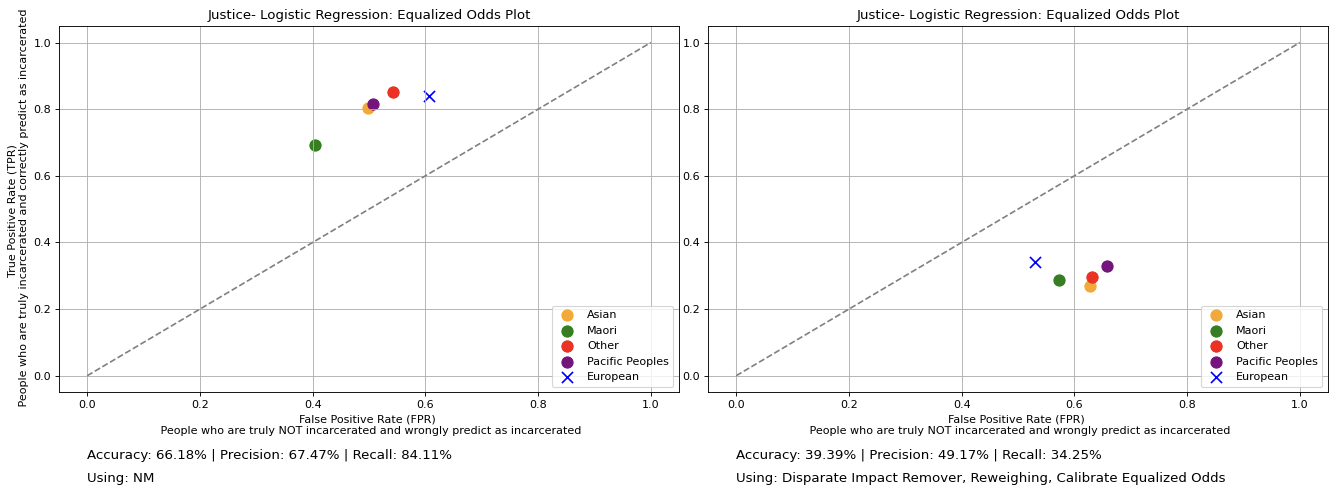
\includegraphics[width=\textwidth]{../tex/justice_eqq}
    \caption{Justice: equalised odds, before/after}
    \label{fig:justice-eqq-mitigations}
\end{figure}

Our results underscore the complexity of balancing fairness and
accuracy in machine learning models. While we achieved our goal of
increasing fairness by mitigating disparity, it came at the
significant cost of accuracy.

As noted in \cite{feldman2015certifying}, this can be a desirable
result when looking at the performance of mitigated models that
exclusively use sensitive attributes: it means the model can no longer
effectively use those attributes to distinguish individuals.

%%%%%%%%%%%%%%%%%%%%%%%%%%%%%%%%%%%%%%%%%%%%%%%%%%%%%%%%%%%%%%%%%%%%%%
\section{Limitations and future work}
\label{sec:limit-future-work}

While the use of AIF360 \cite{bellamy2018ai} accelerated our analysis,
there are several fairness mitigations the library provides that we
did not explore in this study. For example, there are several
in-processing algorithms we did not study.

As previously noted, our datasets have limited features beyond the
offence information. Real world datasets used for training criminal
justice tasks use a much larger number of features. (See for example
\cite{fabris2022algorithmic}.) Our study did not establish whether or
not the effective fairness mitigations we reported would have similar
performance on real world datasets.

These limitations inform avenues for future work: exploring more
fairness mitigations including in-processing techniques referred to
above, and exploring more feature-rich datasets, though that might be
difficult to obtain in the New Zealand context.

In addition, while we focused on disparate impact and equalised odds
in this report, there are many additional fairness metrics that could
be evaluated.


%%%%%%%%%%%%%%%%%%%%%%%%%%%%%%%%%%%%%%%%%%%%%%%%%%%%%%%%%%%%%%%%%%%%%%
\section{Conclusion}
\label{sec:conclusion}

Ensuring the appropriate use of sensitive attributes in machine
learning models is a challenging task and a field of active research.
The task is made more complex by the fact there is no single ``best''
solution applicable to all domains and classification models.

Here we focused on New Zealand criminal data from Police and Ministry
of Justice. In this particular domain, the use of sensitive attributes
such as gender and ethnicity in classification tasks is socially
unacceptable. In other domains, such as medicine, sensitive attributes
may serve as proxies for mechanism that are not otherwise understood
or lack sufficient data, and are actually vital for accurate
modelling. Therefore fair classification techniques are highly
specific to the domain.

Our decision to use publicly available tabular data limited the direct
applicability of our analysis to real-world tasks, but it did allow us
to explore mitigations to the datasets that address the bias present
in the underlying data.

The work we presented can be helpful to government ministries in the
crime and justice domains looking to train machine learning models on
non-public data which includes sensitive attributes, by demonstrating
the bias which exists in the raw data, and the effectiveness of
various fairness mechanisms.

To that end, our report demonstrated that highly accurate models could
be trained to predict severe outcomes solely based on sensitive
attributes. Therefore, mitigations are required if these attributes are
used as part of larger models developed by government.

Our work has demonstrated the challenges of using criminal data in New
Zealand, where the raw datasets aggregated from operational data
encode biases that unmitigated machine learning models will readily
use. We demonstrated the effectiveness of several readily available
fairness mitigations, and contributed a toolkit to allow other
researchers to go further in this domain.

%%%%%%%%%%%%%%%%%%%%%%%%%%%%%%%%%%%%%%%%%%%%%%%%%%%%%%%%%%%%%%%%%%%%%%
\section{Acknowledgements}
\label{sec:acknowledgements}
Thomas Yee, Department of Statistics, University of Auckland, provided
valuable advice regarding the use, interpretation and display of
ethnicity information in the criminal justice domain.

%%%%%%%%%%%%%%%%%%%%%%%%%%%%%%%%%%%%%%%%%%%%%%%%%%%%%%%%%%%%%%%%%%%%%%
\section{Author contributions}
\label{sec:author-contributions}

Garcia structured and implemented the AIF360 toolkit in the fairness
mitigation process. He also contributed with the implementation of
preprocessing strategies and database objects creation. He authored
Section~\ref{sec:our-toolkit} Our toolkit,
Section~\ref{sec:model-implementation} Model implementation.

Omidyar performed data analysis and played a supporting role in the
development and testing of classifiers and mitigations. He authored
Section~\ref{sec:related-work} Related work,
Section~\ref{sec:datasets} Datasets, Section~\ref{sec:data-analysis}
Data analysis, Section~\ref{sec:conclusion} Conclusion, and provided
extensive editing throughout the final report.

Rodriguez spearheaded the efforts in both implementing and evaluating
the mitigation algorithms from the toolkit. He is responsible for the
abstract, Section~\ref{sec:introduction} Introduction, and
Section~\ref{sec:limit-future-work} Limitations and future work.

Xie focused on the mitigation of the two datasets in terms of
preprocessing, explored the effects of different mitigation measures,
wrote the Section~\ref{sec:disparate-impact} Disparate impact,
Section~\ref{sec:equalised-odds} Equalised odds,
Section~\ref{sec:mitigations} Mitigations, and
Section~\ref{sec:ai-fairness-360} AI Fairness 360.

%%%%%%%%%%%%%%%%%%%%%%%%%%%%%%%%%%%%%%%%%%%%%%%%%%%%%%%%%%%%%%%%%%%%%%
\bibliographystyle{splncs04} \bibliography{references}

\end{document}

% LocalWords:  Fabio Omidyar Junjie Xie fgar174 pomi601 lrdo555 Inc
% LocalWords:  jxie936 AIF360 Angwin Northpointe COMPAS scikit etc
% LocalWords:  ANZSOC CEOP FairnessProcessMitigation PRW PDIR json
% LocalWords:  PTCO
